
% This LaTeX was auto-generated from MATLAB code.
% To make changes, update the MATLAB code and republish this document.

\documentclass{article}
\usepackage{graphicx}
\usepackage{color}

\sloppy
\definecolor{lightgray}{gray}{0.5}
\setlength{\parindent}{0pt}

\begin{document}

    
    \begin{verbatim}
clear all
%27
imax = 34;
nmax = 24;
tic;
timedur = toc;
for i=1:imax
    tic;

    if i <= nmax
        [Is(i),pi_me(i),pi_er(i),timepi(i),Vc,points]=Pi_spheref(2^i);
        if i == 14
            figure();
            plot3(Vc(1,points),Vc(2,points),Vc(3,points),'rx');
            hold on;
            plot3(Vc(1,~points),Vc(2,~points),Vc(3,~points),'b.');
            hold off;
            legend('Points in','Points out','Location', 'Best');
            title('MC simulation data for Pi');
        end
    else
        nloops = 2^(i-nmax);
        %disp(num2str(nloops));
        [Ib,pi_meb,pi_erb,timepib,Vcb,pointsb]=Pi_spheref(2^nmax);
        sumbin = sum(pointsb);
        stdbin = std(pointsb);

        parfor ia=2:nloops
            %disp('In loop');
            [Ia,pi_mea,pi_era,timepia,Vca,pointsa]=Pi_spheref(2^nmax);
            %Ib = Ib + Ia;
            sumbin2(ia) = sum(pointsa);
            %stdbin2(ia) = sqrt((stdbin^2+std(pointsa)^2)/2);
            stdbin2(ia) = std(pointsa);
            timepib = timepib+timepia;
            %Vcb = Vcb + Vca;
            %pointsb = pointsb + pointsa;
        end
        sumbin = sumbin + sum(sumbin2);
        stdbin = sqrt((stdbin^2+sum(stdbin2.^2))/nloops);
        Ntotal = 2^i;
        pi_meb = 6*sumbin/(Ntotal);% The calculated values of Pi
        pi_erb = 6*stdbin/sqrt(Ntotal); %The Standard Error of Pi
        [Is(i),pi_me(i),pi_er(i),timepi(i),Vc,points] = deal(Ib,pi_meb,pi_erb,timepib,Vcb,pointsb);

    end
    timedur=toc;
    timerem = timedur*(2^(imax-i+1)-1)/60;
    clc;
    fprintf('%.2f%% Completed, Estimated remaining time %.2f minutes',100*i/imax,timerem);
end

% [I_sorted, I_order] = sort(Is);
% pi_me = pi_me(I_order);
% pi_er = pi_er(I_order);
% timepi = timepi(I_order);

for o=1:imax
    fprintf('Calculated Pi is %.8f with a Standard Error of %.8f and actual Pi is %.8f \n',pi_me(o),pi_er(o),pi);
end

figure();
errorbar(2.^(1:imax),pi_me,pi_er,'o');
title('Calculated value of Pi and errors');
set(gca, 'XScale', 'log');
set(gca, 'YScale', 'log');
xlabel('Number of vectors');
ylabel('Value of Pi');
hold on;
plot([2^1,2^imax],[pi,pi],'r--');
legend('MC Pi','Pi','Location', 'Best');
figure();
yyaxis left;
plot(2.^(1:imax),timepi);
title('Total run time and error');
set(gca, 'XScale', 'log');
set(gca, 'YScale', 'log');
xlabel('Number of vectors');
ylabel('Time calculating Pi (s)');
yyaxis right;
plot(2.^(1:imax),pi_er);
ylabel('Error in Pi');
set(gca, 'YScale', 'log');
legend('Time','Error','Location', 'Best');
\end{verbatim}
\begin{verbatim}
function [M,pi_me,pi_er,timeout,Vc,pointers]=Pi_spheref(N)

%Calculate the value of Pi using MonteCarlo comparing the volumes of a
%sphere and a cube
tic;
%N is the number of random vectros to create
M=N;
Vc = 2*rand(3,N)-1; %The 3D vectors in the (-1,1) region
Norm = sqrt(Vc(1,:).^2+Vc(2,:).^2+Vc(3,:).^2);%Magnitude of vectors
pointers = Norm<1;%The vectros with a magnitude less than 1, inside the sphere
% Vc_in = Vc(pointers);%The positions of the points inside the sphere
% Vc_out = Vc(1-pointers);%The points outside
pi_me = 6*sum(pointers)/N;% The calculate values of Pi
pi_er = 6*std(pointers)/sqrt(N); %The Standard Error of Pi
timeout=toc;
end
\end{verbatim}

        \color{lightgray} \begin{verbatim}2.94% Completed, Estimated remaining time 4252017.62 minutes5.88% Completed, Estimated remaining time 160202.28 minutes8.82% Completed, Estimated remaining time 63851.85 minutes11.76% Completed, Estimated remaining time 55691.41 minutes14.71% Completed, Estimated remaining time 150968.10 minutes17.65% Completed, Estimated remaining time 4178.65 minutes20.59% Completed, Estimated remaining time 1552.45 minutes23.53% Completed, Estimated remaining time 791.88 minutes26.47% Completed, Estimated remaining time 361.27 minutes29.41% Completed, Estimated remaining time 214.75 minutes32.35% Completed, Estimated remaining time 119.40 minutes35.29% Completed, Estimated remaining time 81.37 minutes38.24% Completed, Estimated remaining time 74.45 minutes41.18% Completed, Estimated remaining time 38943.19 minutes44.12% Completed, Estimated remaining time 80.02 minutes47.06% Completed, Estimated remaining time 40.47 minutes50.00% Completed, Estimated remaining time 44.84 minutes52.94% Completed, Estimated remaining time 39.87 minutes55.88% Completed, Estimated remaining time 38.13 minutes58.82% Completed, Estimated remaining time 37.22 minutes61.76% Completed, Estimated remaining time 44.83 minutes64.71% Completed, Estimated remaining time 50.88 minutes67.65% Completed, Estimated remaining time 49.32 minutes70.59% Completed, Estimated remaining time 48.65 minutes73.53% Completed, Estimated remaining time 82.84 minutes76.47% Completed, Estimated remaining time 55.71 minutes79.41% Completed, Estimated remaining time 50.73 minutes82.35% Completed, Estimated remaining time 49.20 minutes85.29% Completed, Estimated remaining time 47.03 minutes88.24% Completed, Estimated remaining time 43.05 minutes91.18% Completed, Estimated remaining time 40.26 minutes94.12% Completed, Estimated remaining time 37.48 minutes97.06% Completed, Estimated remaining time 31.23 minutes100.00% Completed, Estimated remaining time 19.92 minutesCalculated Pi is 6.00000000 with a Standard Error of 0.00000000 and actual Pi is 3.14159265 
Calculated Pi is 1.50000000 with a Standard Error of 1.50000000 and actual Pi is 3.14159265 
Calculated Pi is 3.00000000 with a Standard Error of 1.13389342 and actual Pi is 3.14159265 
Calculated Pi is 4.50000000 with a Standard Error of 0.67082039 and actual Pi is 3.14159265 
Calculated Pi is 2.43750000 with a Standard Error of 0.52925979 and actual Pi is 3.14159265 
Calculated Pi is 3.00000000 with a Standard Error of 0.37796447 and actual Pi is 3.14159265 
Calculated Pi is 3.51562500 with a Standard Error of 0.26224547 and actual Pi is 3.14159265 
Calculated Pi is 3.37500000 with a Standard Error of 0.18639380 and actual Pi is 3.14159265 
Calculated Pi is 3.16406250 with a Standard Error of 0.13251359 and actual Pi is 3.14159265 
Calculated Pi is 3.38085938 with a Standard Error of 0.09303688 and actual Pi is 3.14159265 
Calculated Pi is 3.04980469 with a Standard Error of 0.06629831 and actual Pi is 3.14159265 
Calculated Pi is 3.15673828 with a Standard Error of 0.04681670 and actual Pi is 3.14159265 
Calculated Pi is 3.12304688 with a Standard Error of 0.03311976 and actual Pi is 3.14159265 
Calculated Pi is 3.14794922 with a Standard Error of 0.02340970 and actual Pi is 3.14159265 
Calculated Pi is 3.15673828 with a Standard Error of 0.01655043 and actual Pi is 3.14159265 
Calculated Pi is 3.13751221 with a Standard Error of 0.01170652 and actual Pi is 3.14159265 
Calculated Pi is 3.14328003 with a Standard Error of 0.00827698 and actual Pi is 3.14159265 
Calculated Pi is 3.14435577 with a Standard Error of 0.00585260 and actual Pi is 3.14159265 
Calculated Pi is 3.14720535 with a Standard Error of 0.00413822 and actual Pi is 3.14159265 
Calculated Pi is 3.14473343 with a Standard Error of 0.00292628 and actual Pi is 3.14159265 
Calculated Pi is 3.14034462 with a Standard Error of 0.00206933 and actual Pi is 3.14159265 
Calculated Pi is 3.14305401 with a Standard Error of 0.00146318 and actual Pi is 3.14159265 
Calculated Pi is 3.14205694 with a Standard Error of 0.00103464 and actual Pi is 3.14159265 
Calculated Pi is 3.14044547 with a Standard Error of 0.00073162 and actual Pi is 3.14159265 
Calculated Pi is 3.14145023 with a Standard Error of 0.00051732 and actual Pi is 3.14159265 
Calculated Pi is 3.14125451 with a Standard Error of 0.00036580 and actual Pi is 3.14159265 
Calculated Pi is 3.14145362 with a Standard Error of 0.00025866 and actual Pi is 3.14159265 
Calculated Pi is 3.14208392 with a Standard Error of 0.00018290 and actual Pi is 3.14159265 
Calculated Pi is 3.14140635 with a Standard Error of 0.00012933 and actual Pi is 3.14159265 
Calculated Pi is 3.14149252 with a Standard Error of 0.00009145 and actual Pi is 3.14159265 
Calculated Pi is 3.14168158 with a Standard Error of 0.00006467 and actual Pi is 3.14159265 
Calculated Pi is 3.14157585 with a Standard Error of 0.00004573 and actual Pi is 3.14159265 
Calculated Pi is 3.14157859 with a Standard Error of 0.00003233 and actual Pi is 3.14159265 
Calculated Pi is 3.14159870 with a Standard Error of 0.00002286 and actual Pi is 3.14159265 
\end{verbatim} \color{black}
    
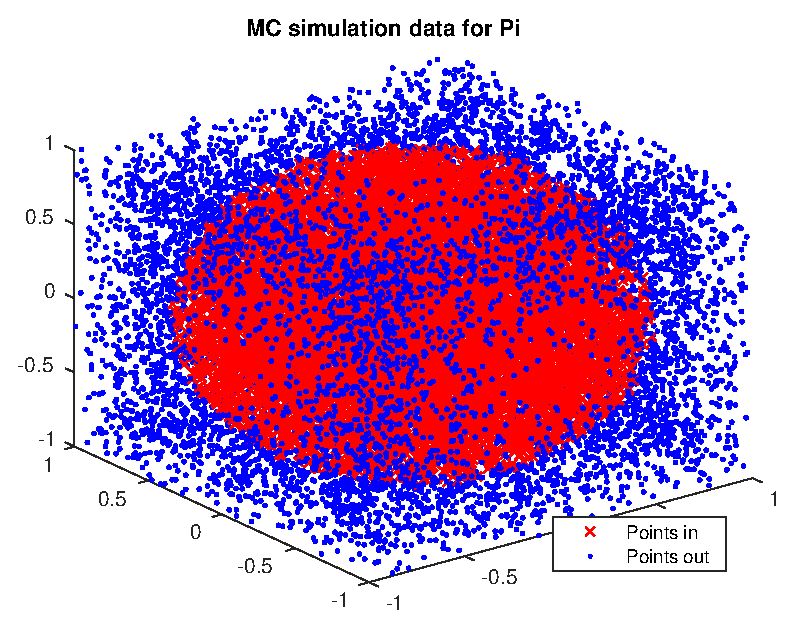
\includegraphics [width=4in]{Pi_sphere_01.eps}

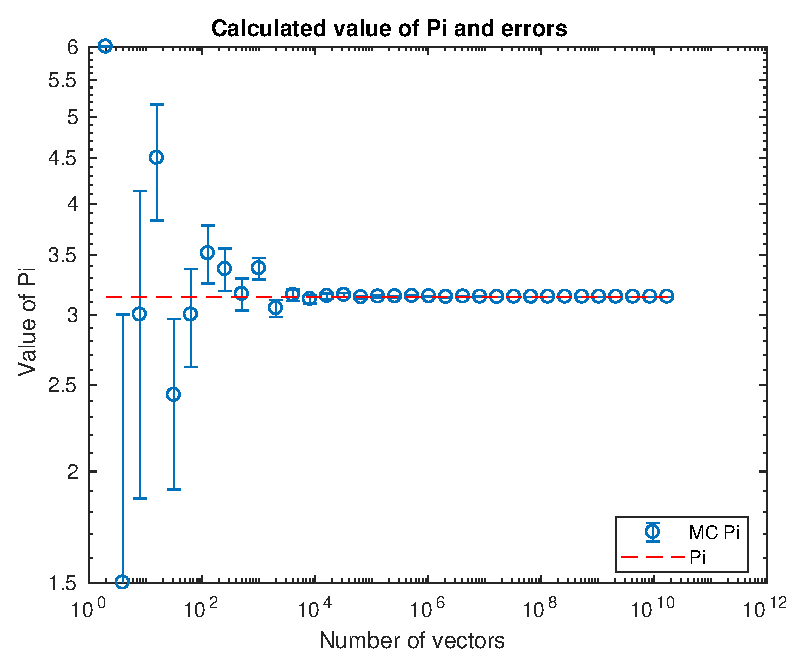
\includegraphics [width=4in]{Pi_sphere_02.eps}

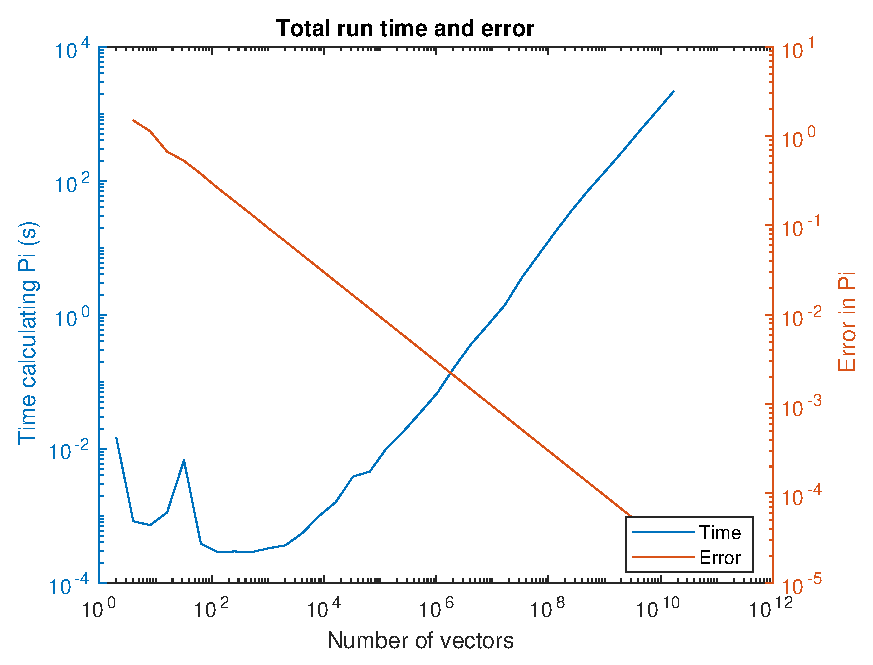
\includegraphics [width=4in]{Pi_sphere_03.eps}



\end{document}
    
